\chapter{平坦坐标中的视界与蒸发的热力学}

\lectureoverview{Schwarzschild 度规在视界处似乎变得奇异，尽管自由下落的观测者在那里不应注意到任何异常。我们通过将近视界度规转换为双曲极坐标下的平坦 Minkowski 空间来解决这一矛盾。同一几何随后将 Alice 的坠落描述与 Bob 的加速外部描述区分开来。后半部分展开熵与温度，推导 Hawking 的逆质量温度与 \(M^3\) 蒸发定律，并以追问信息守恒对引力的微观理论提出什么要求作结。}

\section{\texorpdfstring{\(r=2GM\)}{r=2GM}处的疑难}

从一个非常大的黑洞开始。其视界的曲率可以小到使一个穿过它的观测者在任何适度的实验室尺度区域内看到几乎空无一物的平坦时空。没有墙被撞上，也没有局部警报宣告穿越。然而 Schwarzschild 度规似乎说，恰好在那个半径处发生了某种奇异的事情。本讲前半部分的目的就是使这两个陈述相容。

我们采用 mostly-plus 号差约定。在平坦时空中，
\begin{equation}
ds^2=-dt^2+dx^2+dy^2+dz^2,
\end{equation}
因此类时世界线有 \(ds^2<0\)，固有时满足 \(d\tau^2=-ds^2\)。这是上一讲所用约定整体符号的反转；没有任何可观测量依赖于这一选择。

取 \(c=1\)，Schwarzschild 线元为
\begin{equation}
\begin{aligned}
ds^2={}&-\left(1-\frac{2GM}{r}\right)dt^2
+\frac{dr^2}{1-\frac{2GM}{r}}
+r^2d\Omega_2^2,\\
d\Omega_2^2={}&d\theta^2+\sin^2\theta\,d\phi^2 .
\end{aligned}
\label{eq:l03-schwarzschild}
\end{equation}
Schwarzschild 半径为 \(R_s=2GM\)，或当恢复 \(c\) 时为 \(R_s=2GM/c^2\)。在远处，\(r\gg R_s\)，两个径向系数都趋近其平坦空间值。然而在 \(r=R_s\) 处，\(dt^2\) 的系数为零，而 \(dr^2\) 的系数发散。这看起来颇具戏剧性。问题在于几何本身具有戏剧性，还是仅仅坐标如此。

\section{坐标的两条教训}

\subsection{极坐标的无害起源}

在普通欧几里得平面上，
\begin{equation}
ds^2=dx^2+dy^2.
\end{equation}
引入极坐标
\begin{equation}
x=\rho\cos\theta,
\qquad
y=\rho\sin\theta .
\end{equation}
微小位移的径向长度为 \(d\rho\)，横向长度为 \(\rho\,d\theta\)，因此
\begin{equation}
ds^2=d\rho^2+\rho^2d\theta^2.
\label{eq:l03-polar}
\end{equation}
在 \(\rho=0\) 处，角向系数为零。这并不使平面的中心奇异。它只是说，在那里 \(\theta\) 的每一个值都命名同一个点。因此，一个奇特的度规系数可能诊断的是一个奇特的坐标系，而非奇特的物理。

\subsection{双曲极坐标}

现在把欧几里得平面替换为 \(1+1\) 维 Minkowski 时空，
\begin{equation}
ds^2=-dT^2+dX^2.
\end{equation}
在右手楔形区 \(X>|T|\) 中，定义
\begin{equation}
X=\rho\cosh\omega,
\qquad
T=\rho\sinh\omega,
\qquad \rho>0 .
\label{eq:l03-rindler-transform}
\end{equation}
普通的恒等式 \(\cos^2\theta+\sin^2\theta=1\) 被替换为
\begin{equation}
\cosh^2\omega-\sinh^2\omega=1.
\end{equation}
因此，常 \(\rho\) 线是双曲线
\begin{equation}
X^2-T^2=\rho^2.
\end{equation}
与周期性的角 \(\theta\) 不同，类快度坐标 \(\omega\) 从 \(-\infty\) 延伸到 \(+\infty\)。在大的正 \(\omega\) 处，\(\cosh\omega\) 与 \(\sinh\omega\) 变得几乎相等，双曲线趋近未来零射线 \(X=T\)。

对式~\eqref{eq:l03-rindler-transform}求导给出
\begin{align}
dX&=\cosh\omega\,d\rho+\rho\sinh\omega\,d\omega,\\
dT&=\sinh\omega\,d\rho+\rho\cosh\omega\,d\omega .
\end{align}
交叉项相消，留下
\begin{equation}
ds^2=-\rho^2d\omega^2+d\rho^2.
\label{eq:l03-rindler-metric}
\end{equation}

\begin{figure}[htbp]
\centering
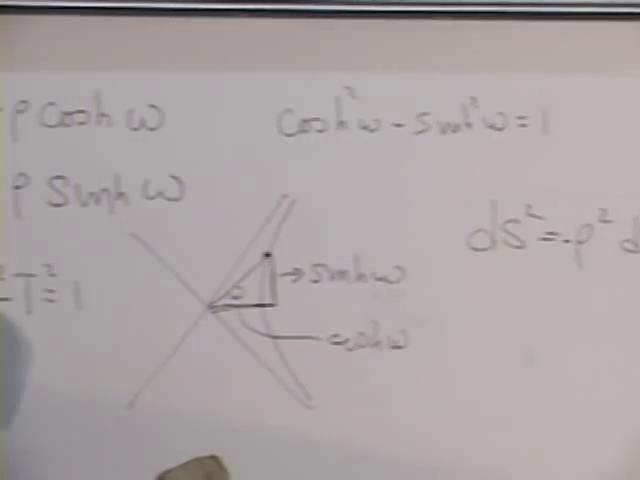
\includegraphics[width=0.72\textwidth]{lecture_03_figure_02.png}
\caption{完成后的双曲坐标板书：\(X=\rho\cosh\omega\)、\(T=\rho\sinh\omega\)、单位双曲线构造，以及形式为 \(ds^2=-\rho^2d\omega^2+d\rho^2\) 的平坦度规。}
\lectureframe{00:16:55.000}
\end{figure}

式~\eqref{eq:l03-rindler-metric}仍然描述完全平坦的时空。其时间系数在 \(\rho=0\) 处为零，正如式~\eqref{eq:l03-polar}的角向系数在原点处为零一样。坐标图在那里退化；时空并不退化。

\section{放大 Schwarzschild 视界}

回到式~\eqref{eq:l03-schwarzschild}的径向-时间部分：
\begin{align}
ds^2
&=-\frac{r-2GM}{r}\,dt^2
+\frac{r}{r-2GM}\,dr^2 .
\label{eq:l03-rewritten-schwarzschild}
\end{align}
我们现在只考察 \(r=2GM\) 的一个狭窄邻域。在变化缓慢的因子中，\(r\) 可以用 \(2GM\) 替换。因子 \(r-2GM\) 必须保留，因为它在视界处为零并改变符号。因此
\begin{equation}
ds^2\approx
-\frac{r-2GM}{2GM}\,dt^2
+\frac{2GM}{r-2GM}\,dr^2 .
\label{eq:l03-near-horizon-r}
\end{equation}

选择一个新的径向坐标 \(\rho\)，使第二项简单地成为 \(d\rho^2\)：
\begin{equation}
d\rho^2=\frac{2GM}{r-2GM}\,dr^2.
\end{equation}
在视界外，取正平方根并从 \(r=2GM\) 积分给出
\begin{align}
d\rho&=\sqrt{\frac{2GM}{r-2GM}}\,dr,\\
\rho&=2\sqrt{2GM}\sqrt{r-2GM},\\
\rho^2&=8GM(r-2GM),
\qquad
r-2GM=\frac{\rho^2}{8GM}.
\label{eq:l03-rho-r}
\end{align}
代入式~\eqref{eq:l03-near-horizon-r}得到
\begin{equation}
ds^2\approx
-\frac{\rho^2}{16G^2M^2}\,dt^2+d\rho^2.
\end{equation}
最后重新标度 Schwarzschild 时间，
\begin{equation}
\omega=\frac{t}{4GM},
\qquad
d\omega^2=\frac{dt^2}{16G^2M^2},
\label{eq:l03-omega}
\end{equation}
并得到
\begin{equation}
\boxed{ds^2\approx-\rho^2d\omega^2+d\rho^2.}
\label{eq:l03-near-horizon-rindler}
\end{equation}

\begin{figure}[htbp]
\centering
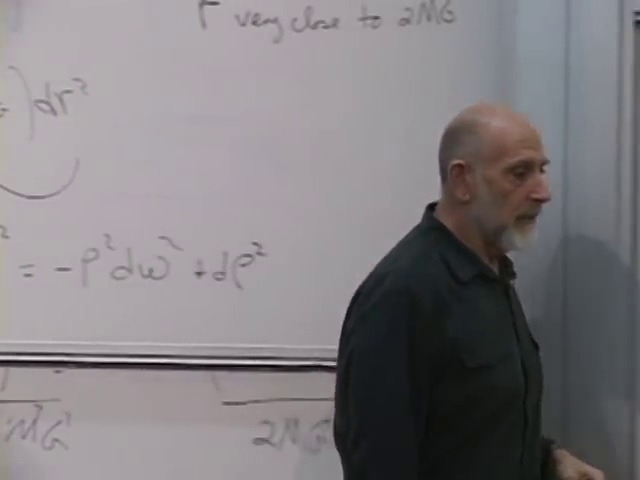
\includegraphics[width=0.70\textwidth]{lecture_03_figure_03.png}
\caption{时间重新标度后的板书：近视界 Schwarzschild 度规已变成与平坦 Minkowski 时空相同的双曲极坐标度规。}
\lectureframe{00:31:35.000}
\end{figure}

当所考察的邻域向视界收缩时，该近似会无限地改善。它证明了我们想要的局部陈述：对于一个足够大的洞，视界就是写在非凡坐标系中的普通时空。对于有限质量的施瓦西洞，曲率并非字面意义上的零，但它在视界处是有限的，并且可以通过增大\(M\)使它在视界处任意小。\editorialnote{局部曲率标度的量级为\(R_s^{-2}\)。林德勒度规是局部近视界展开中的领头项，而不是声称整个施瓦西几何全局平坦。}

\begin{classroomqa}
\audiencequestion{对于\(r<2GM\)，方程~\eqref{eq:l03-rho-r}使这个外部\(\rho\)成为虚数。这是否标志着物理问题？\lecturetimestamp{00:32:30}}
\lecturerresponse{它以不同的形式再现了同样的坐标失效。当前的坐标图是为外部楔形构造的；要延伸穿过视界需要另一个坐标图。这个特定\(\rho\)的失效并不是视界处的物理事件。}
\end{classroomqa}

\begin{classroomqa}
\audiencequestion{在近视界改写中，近似后的线如何从前面的精确线得出？\lecturetimestamp{00:39:21}}
\lecturerresponse{只有\(r\)中缓慢变化的出现被设为等于\(2GM\)。小差值\(r-2GM\)被保留不变。这就是该近似，并且当\(r\)趋近\(2GM\)时它变得越来越精确。}
\end{classroomqa}

\section{坐标的含义}

该变换确认
\begin{equation}
\rho=0\quad\Longleftrightarrow\quad r=2GM.
\end{equation}
外部\(r>2GM\)是右林德勒楔形\(X>|T|\)。恒定\(\rho\)双曲线代表保持在固定施瓦西半径处的观测者。在该楔形中任何地方发出的出射光线都会穿过每一条更大的\(\rho\)世界线，因此外部观测者可以向外通信。未来零边界之外的点无法将光信号发送回右楔形。那条零边界就是视界。

\begin{classroomqa}
\audiencequestion{这里展示的双曲坐标片是否总是描述视界之外的区域？\lecturetimestamp{00:35:22}}
\lecturerresponse{是的。在此构造中\(r>2GM\)给出\(\rho^2>0\)并将事件置于右外部楔形中。零边缘\(\rho=0\)是视界；当前坐标不会作为实外部坐标继续延伸到它之外。}
\end{classroomqa}

\begin{classroomqa}
\audiencequestion{恒定\(\rho\)双曲线代表一个时间还是一个距离？\lecturetimestamp{00:37:21}}
\lecturerresponse{在近视界近似中，它代表到视界的一个固定固有距离，因此也代表一个固定的施瓦西半径。沿双曲线的运动就是驻扎在那里的观测者的时间流逝。}
\end{classroomqa}

沿固定\(\rho\)轨迹，方程~\eqref{eq:l03-rindler-metric}给出
\begin{equation}
d\tau=\rho\,d\omega.
\label{eq:l03-proper-time-rindler}
\end{equation}
因此\(\omega\)本身并不是观测者的固有时间。它是双曲线族共有的角时间；每个观测者将它乘以该观测者的\(\rho\)，正如普通角度乘以圆的半径得到弧长一样。

\begin{classroomqa}
\audiencequestion{\(\omega\)是加速观测者的固有时间吗？\lecturetimestamp{00:51:45}}
\lecturerresponse{几乎是的。在固定\(\rho\)处，固有时间增量为\(\rho\,d\omega\)。\(\rho\)这个因子是必不可少的。}
\end{classroomqa}

\begin{figure}[htbp]
\centering
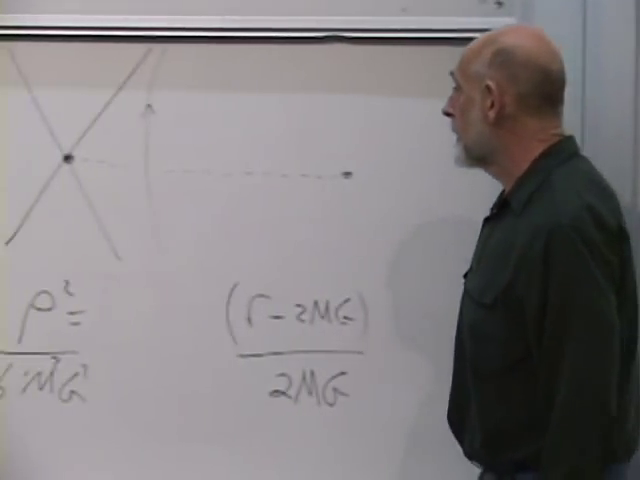
\includegraphics[width=0.72\textwidth]{lecture_03_figure_04.png}
\caption{近视界因果图板：交叉的零边界、外部楔形中的恒定半径双曲线，以及\(\rho\)与\(r-2GM\)之间的坐标关系。}
\lectureframe{00:34:35.000}
\end{figure}

\begin{figure}[htbp]
\centering
\begin{tikzpicture}[scale=1.04,>=Latex]
  \draw[->] (-0.3,0) -- (4.6,0) node[right] {\(X\)};
  \draw[->] (0,-3.2) -- (0,3.2) node[above] {\(T\)};
  \draw[very thick,blue!55!black] (0,0) -- (3,3);
  \draw[very thick,blue!55!black] (0,0) -- (3,-3);
  \node[blue!55!black,rotate=45] at (0.72,1.02) {future horizon};
  \draw[thick,domain=-1.45:1.45,samples=80] plot ({0.75*cosh(\x)},{0.75*sinh(\x)});
  \draw[thick,domain=-1.25:1.25,samples=80] plot ({1.25*cosh(\x)},{1.25*sinh(\x)});
  \draw[very thick,domain=-1.05:1.05,samples=80] plot ({2.0*cosh(\x)},{2.0*sinh(\x)});
  \node at (3.64,2.18) {Bob: \(\rho=\mathrm{const.}\)};
  \draw[very thick,red!65!black,->] (1.2,-2.9) -- (1.2,2.9);
  \node[red!65!black] at (1.58,-1.75) {Alice};
  \fill[red!65!black] (1.2,1.2) circle (1.7pt);
  \draw[dashed,->] (1.2,0) -- (2.27,1.07);
  \node[align=left] at (3.18,0.80) {\small pre-crossing\\[-0.2em]\small light signal};
\end{tikzpicture}
\caption{图板的排版配套图。鲍勃沿一条加速的恒定\(\rho\)双曲线运动；爱丽丝沿一条穿过未来视界的局部惯性线运动。零边界限制了鲍勃的因果可达范围，但并未成为爱丽丝的局部障碍。}
\end{figure}

\section{爱丽丝下落，鲍勃悬停}

让鲍勃保持与视界的固定距离，而爱丽丝松开他的手并下落。鲍勃的世界线是一条双曲线，因此是加速的。爱丽丝的局部世界线近似为直线。她在有限固有时间内穿过零边界，并且不会遇到任何局部不连续性。

因果描述是不对称的。Alice 穿越之后，来自她的光无法到达 Bob，而 Bob 发出的光在一段时间内仍能到达 Alice。Bob 接收到 Alice 在其有限下落入过程中越来越早阶段发出的信号。它们的到达时间间隔越拉越长，频率红移，强度衰减。在 Schwarzschild 时间中，他永远看不到穿越本身；Alice 看起来渐近地趋近并压扁在地平线上。并不是她的鼻子被压扁而后脑勺保持正常：来自每一部分的信号都被压缩进同一个极限层。

\begin{classroomqa}
\audiencequestion{Alice 穿越后能看到 Bob，是因为 Bob 的光子朝她向内传播吗？\lecturetimestamp{00:42:48}}
\lecturerresponse{是的。单向因果关系正是要点：Bob 的向内信号可以进入，而 Alice 后来的向外信号无法逃回 Bob。}
\end{classroomqa}

\begin{classroomqa}
\audiencequestion{如果 Alice 的脚先穿越而她的眼睛仍在外侧，她会暂时看不见自己的脚吗？\lecturetimestamp{00:43:03}}
\lecturerresponse{在普通下落过程中不会出现视觉上的中断。光从脚到眼睛总需要时间；等到相关信号到达时，她的眼睛也已经穿越了。只有猛烈地试图让她的头保持在外侧而脚继续向内，才会造成一种不同且具有破坏性的情形。}
\end{classroomqa}

保持位置是非惯性选择。Bob 需要火箭，正如站在地板上的人需要地板向上的力来避免自由下落。Bob 悬停得越靠近地平线，所需的固有加速度越大；在局部 Rindler 近似中，其大小为 \(a=1/\rho\)，单位为 \(c=1\)。\editorialnote{恢复单位后，对局部 Rindler 观察者给出 \(a=c^2/\rho\)。一个严格静态的 Schwarzschild 观察者的固有加速度在趋近地平线时发散。}

\begin{classroomqa}
\audiencequestion{我们站在报告厅里时是在加速吗？\lecturetimestamp{00:45:40}}
\lecturerresponse{是的，相对于自由下落参考系而言。地板支撑着我们；没有地板，或者没有喷气背包，我们就会下落。}
\end{classroomqa}

\begin{classroomqa}
\audiencequestion{Bob 最终能看到 Alice 位于地平线一个 Planck 长度之内吗？此后会发生什么？\lecturetimestamp{00:49:24}}
\lecturerresponse{正是在那里，经典几何描述不再充分。Planck 长度包含 \(\hbar\)，因此回答 Bob 在那里能分辨什么需要量子力学。}
\end{classroomqa}

\begin{classroomqa}
\audiencequestion{等半径曲线似乎以类似直角的坐标拐角与地平线相交。那里能取导数吗？\lecturetimestamp{00:51:12}}
\lecturerresponse{在这个点上，该坐标图确实发生了某种奇异的事情，但局部物理没有。覆盖其他楔区的坐标图会消除这个人为拐角。对于当前的外部讨论，Rindler 图像已经包含了所需的因果事实。}
\end{classroomqa}

因此，不指明观察者就问 Alice 是否\emph{真的}穿越了，是没有帮助的。Alice 的时钟在有限固有时间内到达地平线。Bob 接收到的信号序列从不包含穿越事件。物理学问的是每个观察者测量到什么，以及他们的记录如何比较。

\begin{classroomqa}
\audiencequestion{确切的陈述是 Bob 只能看到 Alice 未来的一有限部分，尽管他自己的观测时间无界吗？\lecturetimestamp{00:53:33}}
\lecturerresponse{是的。Alice 为她下落中可见的那部分分配了有限的固有时间。在理想化的永恒几何中，Bob 永远接收到其越来越延迟且红移的信号，但他看不到她在地平线穿越之后继续变老。}
\end{classroomqa}

\section{加速视界已经足够}

这一因果结构中没有任何东西需要黑洞。一个永远匀加速的火箭在平直时空中沿 Rindler 双曲线运动，并具有一个零边界，超过它任何信号都无法追上该火箭。对该观察者而言存在一个加速视界，尽管惯性观察者把同一区域视为普通的 Minkowski 空间。

\begin{classroomqa}
\audiencequestion{这一现象是黑洞特有的，还是对任何视界都会发生？\lecturetimestamp{00:55:25}}
\lecturerresponse{同一现象对匀加速观察者也会发生。这样的观察者有一个加速视界，看不到其外的事件。局部地看，黑洞视界与那种情形在物理上没有不同。}
\end{classroomqa}

这就是等效原理在起作用：先理解匀加速，然后在引力场中辨认出相同的局部结构。事后看来，甚至在黑洞被接受之前，人们本可以从加速视界预见到引力视界。爱因斯坦本人并不接受黑洞的物理形成，尽管正是他提供了其几何所由之导出的理论。视界对自由下落的观测者是乏味的，而对坚持留在外面的观测者则意义重大。这是两种有效描述之间的张力，尚不是悖论。

\section{回到热与熵}

休息之后，戴上热力学的帽子。在先前的构造中，黑洞像浴缸一样被一滴一滴地填满，只不过每一滴都是携带大约一个比特的光子。每个比特使视界面积增加一个普朗克面积量级的量。精确的熵为
\begin{equation}
S_{\mathrm{BH}}=\frac{k_B A}{4\ell_P^2}.
\end{equation}
讲座开玩笑说，如果普朗克当初以不同方式定义他的长度，因子\(1/4\)本可以避免。严肃的要点是，量纲分析确定了尺度，但没有确定数值系数；霍金的计算确定了系数。\editorialnote{普朗克长度有一个标准定义\(\ell_P=\sqrt{G\hbar/c^3}\)。一旦固定了这一约定和通常的热力学熵，因子\(1/4\)就是物理的；关于重新定义它的说法只是关于约定的课堂玩笑。}

温度感觉起来很基本，因为手指和温度计直接记录它。熵往往感觉更神秘。讲座颠倒了这一等级：熵和能量被当作基本变量，而温度则从熵变化时能量必须改变多少导出：
\begin{equation}
dE=T\,dS.
\end{equation}
在讲座的一个比特单位中，\(\Delta S=1\)，因此与增加或擦除一个比特相关的最小能量被称为\(T\)。粗心地擦除---用逻辑上相当于大锤的方式---可以耗散任意更多的能量。该定义关注的是当缺失的信息被转移到微观环境自由度中时可能的最小耗散。在常规单位中，一个二进制比特携带\(\Delta S=k_B\ln2\)，而可逆擦除至少耗散\(k_BT\ln2\)。\editorialnote{这就是讲座选择以基于能量的自然单位来测量熵和温度所压制的兰道尔归一化。}

\subsection{单光子估计}

选择一个波长与史瓦西半径相当的光子：
\begin{equation}
\lambda\sim R_s=\frac{2GM}{c^2}.
\end{equation}
在区分\(h\)与\(\hbar\)的\(2\pi\)约定下，其能量为
\begin{equation}
\Delta E\sim \frac{\hbar c}{\lambda}.
\end{equation}
这就是所增加比特的能量代价，所以
\begin{equation}
k_BT_H\sim\frac{\hbar c}{R_s}
\sim\frac{\hbar c^3}{GM}.
\label{eq:l03-hawking-scale}
\end{equation}
启发式论证无法确定诸如\(2\)和\(\pi\)这样的因子。精确的霍金结果是
\begin{equation}
\boxed{k_BT_H=\frac{\hbar c^3}{8\pi GM}.}
\label{eq:l03-hawking-exact}
\end{equation}

\begin{figure}[htbp]
\centering
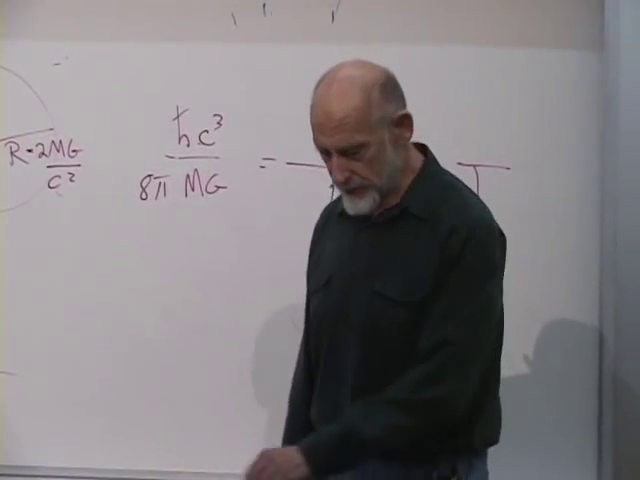
\includegraphics[width=0.72\textwidth]{lecture_03_figure_05.png}
\caption{完成的温度板书：\(R_s=2GM/c^2\)、一个比特尺度\(\hbar c/R_s\)，以及精确的\(8\pi\)霍金归一化。}
\lectureframe{01:07:48.000}
\end{figure}

两个事实立刻可见。第一，温度随\(\hbar\)而消失，所以它是一种量子效应。第二，
\begin{equation}
T_H\propto\frac{1}{M}.
\end{equation}
大黑洞是冷的。对于一个太阳质量，
\begin{equation}
T_H\approx6\times10^{-8}\ {\rm K},
\end{equation}
这与讲座的\(10^{-8}\,\mathrm{K}\)估计处于同一量级，并远低于约\(2.7\,\mathrm{K}\)的宇宙微波背景温度。

\subsection{负热容}

把这样的黑洞放入更暖的环境中。它吸收能量，质量增加，而方程~\eqref{eq:l03-hawking-exact}表明它变得更冷。于是它更容易继续吸收。把它放入更冷的环境中，则反向的失控开始：它辐射，失去质量，变得更热，并辐射得更快。形式上，
\begin{equation}
C_{\mathrm{BH}}
=\frac{dE}{dT_H}
=c^2\frac{dM}{dT_H}
<0.
\end{equation}

\begin{classroomqa}
\audiencequestion{这就是负比热的意思吗？\lecturetimestamp{01:14:08}}
\lecturerresponse{正是。一个自引力系统可以在失去能量时升温。恒星做类似的事情：当它辐射时，降低的压力使它收缩，而引力压缩提高其温度。}
\end{classroomqa}

孤立黑洞并不因此就是非物理的。在当今宇宙中，恒星级黑洞比其周围更冷，并主要吸收。随着宇宙膨胀和背景冷却，平衡最终可能反转，蒸发可能占主导。与有效无限热浴的简单平衡是不稳定的。\editorialnote{边界条件很重要。黑洞可以在有限反射腔中稳定下来，或者对于适当的大黑洞，在反德西特时空中稳定下来；这里描述的不稳定性是渐近平直、普通热浴的情形。}

\section{蒸发定律}

对于标度推导，设想手边没有参考书，选择使所记住的方程最为简洁的单位：
\begin{equation}
c=\hbar=G=k_B=1.
\end{equation}
这些就是普朗克单位。讲座中给出的特征尺度为
\begin{equation}
\ell_P\sim10^{-35}\ {\rm m},
\qquad
t_P\sim10^{-43}\ {\rm s},
\qquad
m_P\sim10^{-8}\ {\rm kg}.
\end{equation}
普朗克质量大致相当于一粒可见的尘埃，而普朗克长度和时间则极其微小。由于\(c=1\)，\(t_P\)不过是\(\ell_P\)的光穿越时间。

把黑洞视为黑体，即一个热辐射体，而不是一个必须保持完全黑暗的物体。它可以发射电磁辐射，原则上还可以发射其他可用的粒子种类，包括引力子。辐射功率与发射面积成正比，因为辐射是通过表面离开的。斯特藩--玻尔兹曼标度关系为
\begin{equation}
L=-\frac{dE}{dt}\sim A T^4.
\end{equation}
在普朗克单位下，\(E=M\)，\(R_s\sim M\)，\(A\sim R_s^2\sim M^2\)，\(T\sim R_s^{-1}\sim M^{-1}\)。因此
\begin{align}
-\frac{dM}{dt}
&\sim R_s^2\left(\frac{1}{R_s}\right)^4
\sim\frac{1}{R_s^2}
\sim\frac{1}{M^2},\\
-M^2\frac{dM}{dt}&\sim1,\\
-\frac{d(M^3)}{dt}&\sim1.
\label{eq:l03-evap-scaling}
\end{align}
忽略量级为1的系数，寿命为
\begin{equation}
\boxed{t_{\mathrm{evap}}\sim M^3.}
\label{eq:l03-lifetime}
\end{equation}

\begin{figure}[htbp]
\centering
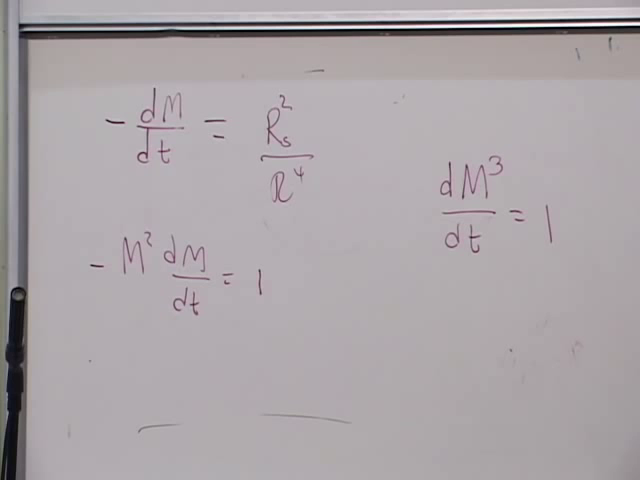
\includegraphics[width=0.72\textwidth]{lecture_03_figure_06.png}
\caption{畅通无阻的蒸发图景：光度给出\(-dM/dt\sim1/M^2\)，因此\(M^3\)均匀减小，寿命与初始质量的立方成正比。}
\lectureframe{01:23:20.000}
\end{figure}

这种示意性的斯特藩--玻尔兹曼处理忽略了灰体因子和粒子种类的数目。对于最简单的无质量发射近似下的中性、不转动黑洞，恢复常数后得到
\begin{equation}
t_{\mathrm{evap}}
=\frac{5120\pi G^2M_0^3}{\hbar c^4}.
\label{eq:l03-exact-lifetime}
\end{equation}
这个系数是编者补充的；讲座只推导稳健的\(M_0^3\)依赖关系。

\subsection{太阳、山岳与千克尺度}

太阳的质量为\(M_\odot\sim10^{30}\,\mathrm{kg}\sim10^{38}m_P\)。取立方并乘以一个普朗克时间，得到讲座中有意粗略的推导链
\begin{equation}
t_{\mathrm{evap}}\sim10^{114}t_P
\sim10^{71}\ {\rm s}
\sim10^{64}\ {\rm yr}.
\end{equation}
两种估计都比宇宙大约\(10^{10}\)年的年龄长得不可思议。恢复方程~\eqref{eq:l03-exact-lifetime}中的系数后，标准的太阳质量估计值提高到约\(2\times10^{67}\)年。\editorialnote{这一差异是意料之中的：黑板上的计算丢弃了所有数值常数，并将普朗克尺度按10的幂次取整。其目的是展示质量立方标度关系，而非精确的寿命天文学。}

接下来课堂上尝试了一个\emph{山岳质量}的黑洞。他们确定了粗略的课堂数值\(M\sim10^{10}\,\mathrm{kg}\)，因此\(M\sim10^{18}m_P\)，并得到
\begin{equation}
t_{\mathrm{evap}}\sim10^{54}t_P
\sim10^{11}\ {\rm s}
\sim10^4\ {\rm yr}.
\end{equation}
这保留了黑板上实际进行的算术。用来引出该质量的言语几何描述---大约\(100\,\mathrm{km}^3\)的岩石---实际上会重得多，而精确的寿命系数也会显著改变结果。\editorialnote{在普通岩石密度下，\(100\,\mathrm{km}^3\)的量级为\(10^{14}\,\mathrm{kg}\)，而非\(10^{10}\,\mathrm{kg}\)。对于\(10^{10}\,\mathrm{kg}\)，方程~\eqref{eq:l03-exact-lifetime}给出的寿命量级为\(10^6\)年。这些修正并不改变讲座的教训：寿命随质量的立方下降。}

\begin{classroomqa}
\audiencequestion{质量只有一千克的黑洞会极其微小吗？\lecturetimestamp{01:29:14}}
\lecturerresponse{是的。由于半径与质量成正比，而一个太阳质量对应几千米，所以一千克的黑洞的施瓦西半径约为\(10^{-27}\,\mathrm{m}\)。这样的黑洞也会极其炽热且寿命极短。}
\end{classroomqa}

\begin{classroomqa}
\audiencequestion{这些蒸发估计是否假设环境温度为零？\lecturetimestamp{01:29:53}}
\lecturerresponse{它们适用于周围环境比黑洞更冷、因而净能量向外流动的情形。更热的环境反而会向黑洞供给能量。霍金温度与当前背景温度相匹配的质量留作练习。}
\end{classroomqa}

为了便于定位，令\(T_H=2.7\,\mathrm{K}\)，得到\(M\)的量级为\(10^{22}\,\mathrm{kg}\)，施瓦西半径的量级为\(10^{-4}\,\mathrm{m}\)。\editorialnote{这是对讲座中所提练习的解答；它不属于口头推导的一部分。}

\section{度规之下必须有什么？}

\begin{classroomqa}
\audiencequestion{是什么机制使光子从黑洞中出来？\lecturetimestamp{01:30:53}}
\lecturerresponse{在给出辐射的微观机制之前，必须先确定负责熵的自由度。热力学论证约束了必须存在什么，但尚未明确展示那些变量。}
\end{classroomqa}

类比是流体力学。流体动力学描述光滑的密度场和速度场，而不追踪每一个分子。然而熵揭示出，许多隐藏的微观组态构成了同一个光滑状态的基础。同样地，经典广义相对论描述光滑的度规，却不暴露黑洞熵所计数的众多微观自由度。面积定律和霍金辐射是线索，表明爱因斯坦的理论是一种有效的宏观描述。

\begin{classroomqa}
\audiencequestion{如果黑洞辐射能量，这是否等同于说它辐射信息，从而在增长过程中被吞入的信息会在蒸发过程中返回？\lecturetimestamp{01:33:27}}
\lecturerresponse{这正是要求所在：如果完整的演化守恒信息，那么出射辐射最终必须能够区分形成该黑洞的各种可能状态。这仍须与物质穿过视界的因果图像相协调。}
\end{classroomqa}

仅凭能量通量不足以确定信息。一个完全热化的密度矩阵可以携带能量，却遗忘详细的初始状态。在幺正描述中，所需的信息编码于发射量子之间的精细关联之中。\editorialnote{这一区分明确揭示了信息问题的现代形式。它使讲座中提出的问题更加尖锐，而非改变该问题。}

\section{信息守恒作为结构性原理}

\begin{classroomqa}
\audiencequestion{信息守恒真的是一条基本原理吗？\lecturetimestamp{01:34:13}}
\lecturerresponse{它属于最根本的原理之列。如果不同的初始状态能够演化到完全相同的末态，那么定律就会抹去自身的过去。通常的守恒定律不仅依赖于对称性，还依赖于可逆的哈密顿量或幺正形式的演化。}
\end{classroomqa}

如讲座中那样，设想一条虚构的基本定律，它只是让每一块滑动的橡皮都停下来。不同的初始速度最终都终结于同一状态。末态的橡皮不再能区分它的历史：信息已被摧毁。动量和机械能也一并消失。真实的摩擦在微观层面并不会如此；动量和能量会传入桌面、空气和热自由度之中。

即便是一个完全均匀的无限大桌面，也会具有平移对称性，然而那条虚构的阻尼定律仍能使橡皮停下。因此，仅凭平移对称性并不足以从这样一条非哈密顿规则导出动量守恒。诺特定理假定了一个作用量原理以及与之相关的可逆动力学。用这里使用的语言来说，对称性加上保信息的动力学才给出守恒定律。

\begin{classroomqa}
\audiencequestion{信息守恒比因果性更根本吗？\lecturetimestamp{01:37:00}}
\lecturerresponse{它们是处于相当的基础层面上的不同原理。因果性必须首先被精确陈述---例如，信号不能逆着传播到允许的因果结构之外---但这两个原理都不能简单地取代另一个。}
\end{classroomqa}

\begin{classroomqa}
\audiencequestion{哈密顿力学中讨论的相空间面积保持，是这一思想的经典版本吗？\lecturetimestamp{01:37:38}}
\lecturerresponse{是的。刘维尔定理说，哈密顿流保持相空间体积。一团可能的初始状态不能坍缩到更小的体积中并抹去区分。在量子力学中，相应的陈述是幺正性：内积，从而正交状态之间的区分，都得到保持。}
\end{classroomqa}

经典地，
\begin{equation}
\frac{d}{dt}\,\mathrm{Vol}_{\Gamma}=0,
\end{equation}
对于由哈密顿流输运的相空间区域。量子力学地，
\begin{equation}
\begin{aligned}
\ket{\psi(t)}&=U(t)\ket{\psi(0)},\\
U^\dagger U&=I,\\
\braket{\psi(t)}{\phi(t)}
&=\braket{\psi(0)}{\phi(0)}.
\end{aligned}
\end{equation}
这些是“微观区分在时间演化中得以存留”这一主张的精确形式。

\section{熵依赖于哪个方向？}

最后的交流回到信息论熵。给定微观备选情形的概率\(p_i\)，
\begin{equation}
S=-k_B\sum_i p_i\ln p_i
\label{eq:l03-shannon}
\end{equation}
以热力学单位表示，或者去掉\(k_B\)后得到无量纲的香农熵。

\begin{figure}[htbp]
\centering
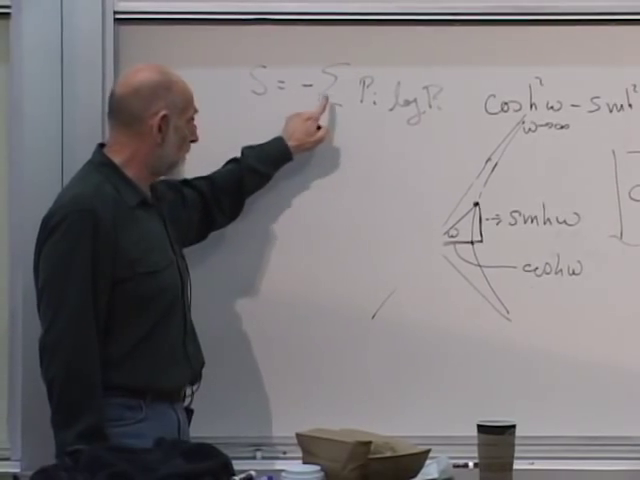
\includegraphics[width=0.72\textwidth]{lecture_03_figure_07.png}
\caption{结尾的板书公式\(S=-\sum_i p_i\log p_i\)，书写时区分了概率分布与由它计算出的单个熵值。}
\lectureframe{01:40:32.000}
\end{figure}

\begin{classroomqa}
\audiencequestion{是最大化熵定义了概率分布，而不是概率定义了熵吗？\lecturetimestamp{01:38:33}}
\lecturerresponse{一个概率分布通过式~\eqref{eq:l03-shannon}确定一个熵值；一个数无法重构所有的\(p_i\)。只有在归一化以及其他约束，例如固定的平均能量，也已被给出之后，最大化熵才能选出一个分布。}
\end{classroomqa}

这一区分使讲座恰好在正确的前沿结束。光滑几何引出了视界；视界引出了热力学；热力学暴露了隐藏的自由度；而信息守恒现在要求这些自由度在演化时不抹去进入黑洞的那些区分。机制尚未给出。相反，几何与记账已经清楚表明，任何成功的微观理论都必须解释什么。
